\section{Segmentación}

\subsection{Introducción}

En esta segunda práctica se ha estudiado un problema con datos sobre  \href{https://sedeapl.dgt.gob.es/WEB_IEST_CONSULTA/subcategoria.faces}{\textit{accidentes de tráfico}} de la Dirección General de Tráfico(DGT) en el año 2013. Los datos recogidos por la DGT contienen variables que caracterizan los accidentes, y se intentará encontrar grupos de accidentes similares dentro del dataset. Estos datos incluyen información entre los años 2008 y 2013, además de más de 30 variables. Nuestro dataset contendrá las siguientes variables, entre otras:

\begin{itemize}
\item MES
\item HORA
\item DIASEMANA
\item PROVINCIA
\item COMUNIDAD\_AUTONOMA
\item TOT\_VICTIMAS
\item TOT\_MUERTOS
\item TOT\_HERIDOS\_GRAVES
\item TOT\_HERIDOS\_LEVES
\item TIPO\_VIA
\item TIPO\_INTERSEC
\item PRIORIDAD
\item LUMINOSIDAD
\item TIPO\_ACCIDENTE
\item DENSIDAD\_CIRCULACION
\end{itemize}

Para abordar esta práctica he usado los siguientes algoritmos:

\begin{itemize}
\item K-Means(Partitional)
\item Agglomerative Clustering(Hierarchical)
\end{itemize}

A pesar de que el método jerárquico no necesita un valor de $k$ , se lo paso para comparar con los obtenidos con K-Means para ese mismo de valor de $k$ y porque en tiempo de ejecución será menos costoso.

\subsection{Caso de estudio 1}

El primer caso de estudio está relacionado con el tipo de intersección sobre el que se produce el accidente. Tenía interés sobre las salidas ya que pensé que quizás en salidas de autovía(por la velocidad que se circula en estas aun cruzando por poblado) y otro tipos de vías se verían diferencias en los accidentes que se producirían. Además, en mi pueblo habitual, se hicieron unos pasos de peatones en la propia salida de una y siempre me pareció algo bastante peligroso.

\subsubsection{Tipo de intersección - Enlace de salida}


Lo primero que pude ver es que la mayoría de accidentes se producen en autovía, asi que podría responder la pregunta que me estaba haciendo; seguidos de ramal de enlace, con autopista y via convecional con cifras similares.

\begin{figure}[H]
\centering
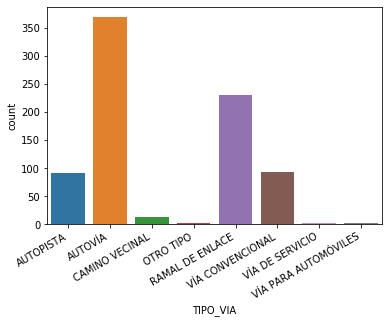
\includegraphics[width=0.5\textwidth]{imagenes/tipo_via_caso1.png}
\caption{Tipo de vía en intersecciones de tipo 'enlace de salida'}
\end{figure}

Viendo las victimas totales de los accidentes que se producen pense inmediatamente que se tratarían de atropellos, cosa que pude comprobar al mirar los tipos de accidentes de los que se trataban. La gran mayoría de animales sueltos y en mucha menor cantidad de peatones, también suman bastantes los casos de colisión con obstáculos seguido de colisiones de vehículos. También se puede apreciar una importante cantidad de accidentes por salida de vía(cosa que me llama la atención por un \href{http://www.dgt.es/es/prensa/notas-de-prensa/2014/20140103-balance-2013-seguridad-vial-2013.shtml}{\textit{artículo}} que leí de la DGT que decía que el tipo de accidente que registra más fallecidos, es de este tipo).

\begin{figure}[H]
\begin{subfigure}{.5\textwidth}
  \centering
  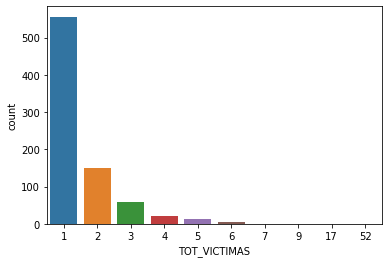
\includegraphics[width=0.8\textwidth]{imagenes/victimas_caso1.png}
  \caption{Número de victimas en intersecciones de tipo 'enlace de salida'}
  \label{fig:sfig1}
\end{subfigure}%
\begin{subfigure}{.5\textwidth}
  \centering
  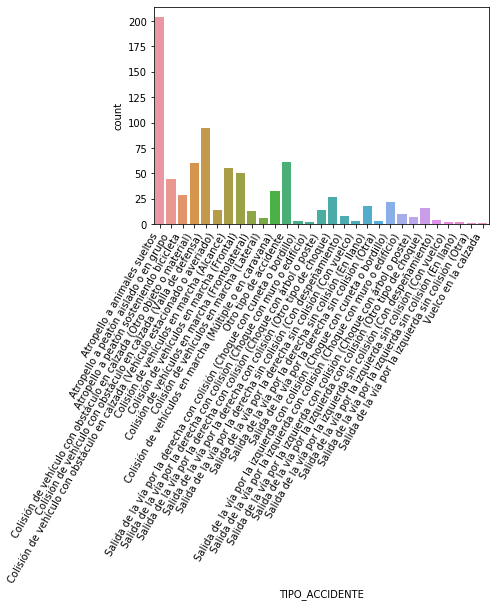
\includegraphics[width=0.8\textwidth]{imagenes/tipo_accidente_caso1.png}
  \caption{Tipo de accidentes en intersecciones de tipo 'enlace de salida'}
  \label{fig:sfig2}
\end{subfigure}
\caption{Víctimas y tipos de accidente en intersecciones de tipo 'enlace de salida'}
\label{fig:fig}
\end{figure}

\paragraph{Resultados de la segmentación}

Para aplicar clustering he usado valores de $k\in[3,7]$, ya que no quería probar con valores grandes de $k$.

Para evaluar la calidad del agrupamiento obtenido, se usarán las siguientes medidas:
\begin{itemize}
\item Coeficiente de Silhouette: nos dice cómo de similares son los objetos de un mismo cluster comparado con otros clusters.

\begin{figure}[H]
\centering
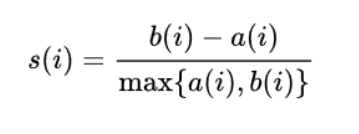
\includegraphics[width=0.35\textwidth]{imagenes/sil.png}
\end{figure}

Sea $a(i)$ la distancia media del objeto $i$ al resto de objetos de su cluster. Sea $b(i)$ la mínima distancia media del objeto $i$ al resto de objetos del resto de clusters. Toma valores en [-1,1], cuanto más cercano a 1, mejor agrupados están los clusters.

La media de todos los $s(i)$ es el coeficiente silhoutteque mide la calidad global del agrupamiento.

\item Índice de Calisnki-Harabasz: razón entre la dispersión intra-cluster y la dispersión inter-cluster. Cuanto mayor es el valor, mejor es el agrupamiento.

\begin{figure}[H]
\centering
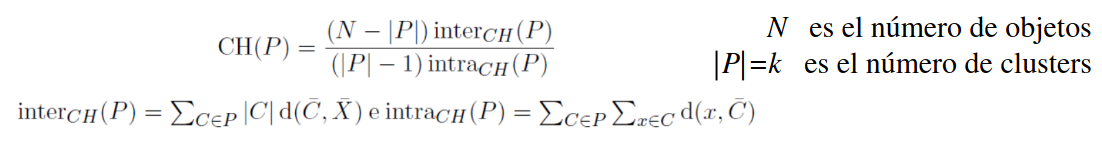
\includegraphics[width=\textwidth]{imagenes/calinski.png}
\end{figure}

\end{itemize}


\begin{table}[H]
%1
\begin{subtable}[H]{0.45\textwidth}
        \centering
\begin{tabular}{|c|c|c|}
\hline
\textit{k = 3}      & \textbf{K-Means}           & \textbf{Agg-Clustering}  \\ \hline
\textbf{Silhouette} & \textit{0,6214}            & \textit{\textbf{0,6231}} \\ \hline
\textbf{Calinski}   & \textit{\textbf{293,1046}} & 283,6044                 \\ \hline
\end{tabular}
\end{subtable}
\hfill
\begin{subtable}[H]{0.45\textwidth}
        \centering
\begin{tabular}{|c|c|c|}
\hline
\textit{k = 4}      & \textbf{K-Means}           & \textbf{Agg-Clustering}  \\ \hline
\textbf{Silhouette} & \textit{0,6584}            & \textit{\textbf{0,6590}} \\ \hline
\textbf{Calinski}   & \textit{\textbf{335,2021}} & 333,9225                 \\ \hline
\end{tabular}
\end{subtable}
%2
\begin{subtable}[H]{0.45\textwidth}
        \centering
\begin{tabular}{|c|c|c|}
\hline
\textit{k = 5}      & \textbf{K-Means}           & \textbf{Agg-Clustering}  \\ \hline
\textbf{Silhouette} & \textit{0,6663}            & \textit{\textbf{0,6668}} \\ \hline
\textbf{Calinski}   & \textit{\textbf{433,5601}} & 431,6778                 \\ \hline
\end{tabular}
\end{subtable}
\hfill
\begin{subtable}[H]{0.45\textwidth}
        \centering
\begin{tabular}{|c|c|c|}
\hline
\textit{k = 6}      & \textbf{K-Means}           & \textbf{Agg-Clustering} \\ \hline
\textbf{Silhouette} & \textit{\textbf{0,7593}}   & \textit{0,7586}         \\ \hline
\textbf{Calinski}   & \textit{\textbf{656,0137}} & 643,6053                \\ \hline
\end{tabular}
\end{subtable}
%3
\begin{subtable}[H]{0.45\textwidth}
        \centering
\begin{tabular}{|c|c|c|}
\hline
\textit{k = 7}      & \textbf{K-Means}           & \textbf{Agg-Clustering}  \\ \hline
\textbf{Silhouette} & \textit{0,7810}            & \textit{\textbf{0,7817}} \\ \hline
\textbf{Calinski}   & \textit{\textbf{844,7296}} & 825,1405                 \\ \hline
\end{tabular}
\end{subtable}
\hfill
\caption{Resultados obtenidos con los distintos algoritmos para las intersecciones de tipo 'enlace de salida'}
\end{table}


Como podemos ver en cuanto al valor de Silhouette, ambos algoritmos han estado a la par, por lo que poco podemos sacar de él. En cuanto a Calinski, se puede ver como siempre con K-Means se obtiene mejor resultado. 

Con estos datos, el mejor agrupamiento se realiza con $k=7$ de los que he probado. A mayor valor de $k$, mejor es este segun el índice Calinski.

Parece que seguirá creciendo mientras crece $k$, pero ya empezarían a dar demasiados numeros de clusters.


\paragraph{Interpretación de la segmentación}

\begin{figure}[H]
\begin{subfigure}{.5\textwidth}
  \centering
  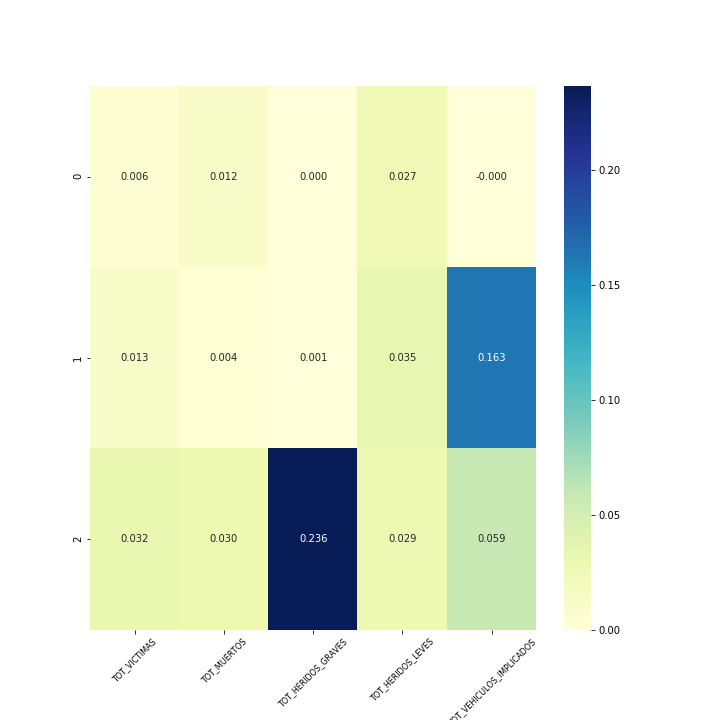
\includegraphics[width=0.9\textwidth]{imagenes/case1/kmeans/heatmaps/hm_kmeans_case1_salida_k3.png}
\end{subfigure}%
\begin{subfigure}{.5\textwidth}
  \centering
  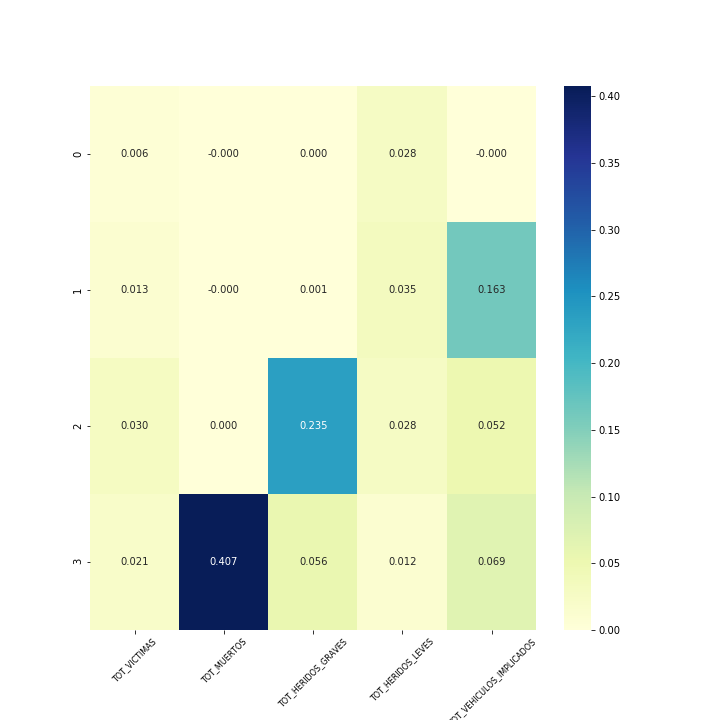
\includegraphics[width=0.9\textwidth]{imagenes/case1/kmeans/heatmaps/hm_kmeans_case1_salida_k4.png}
\end{subfigure}
\begin{subfigure}{.5\textwidth}
  \centering
  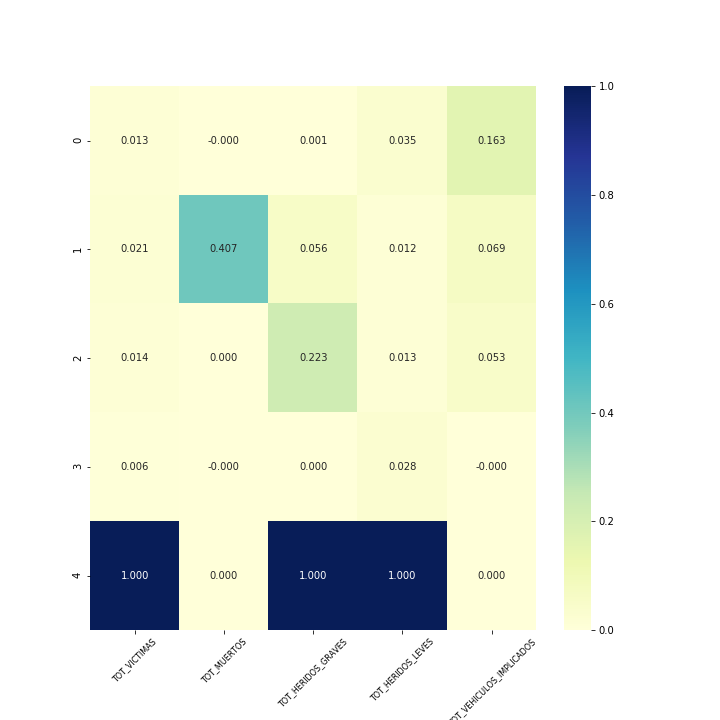
\includegraphics[width=0.9\textwidth]{imagenes/case1/kmeans/heatmaps/hm_kmeans_case1_salida_k5.png}
\end{subfigure}
\begin{subfigure}{.5\textwidth}
  \centering
  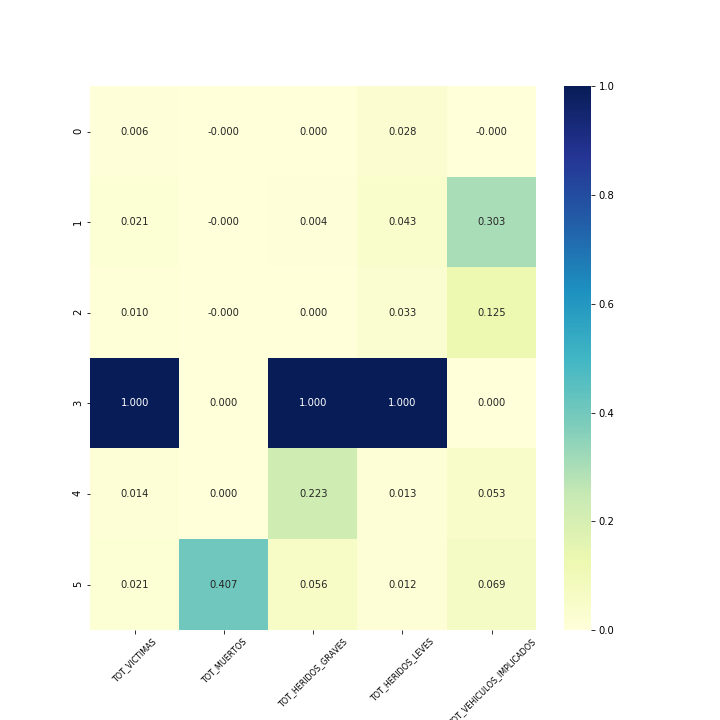
\includegraphics[width=0.9\textwidth]{imagenes/case1/kmeans/heatmaps/hm_kmeans_case1_salida_k6.png}
\end{subfigure}
\begin{subfigure}{.5\textwidth}
  \centering
  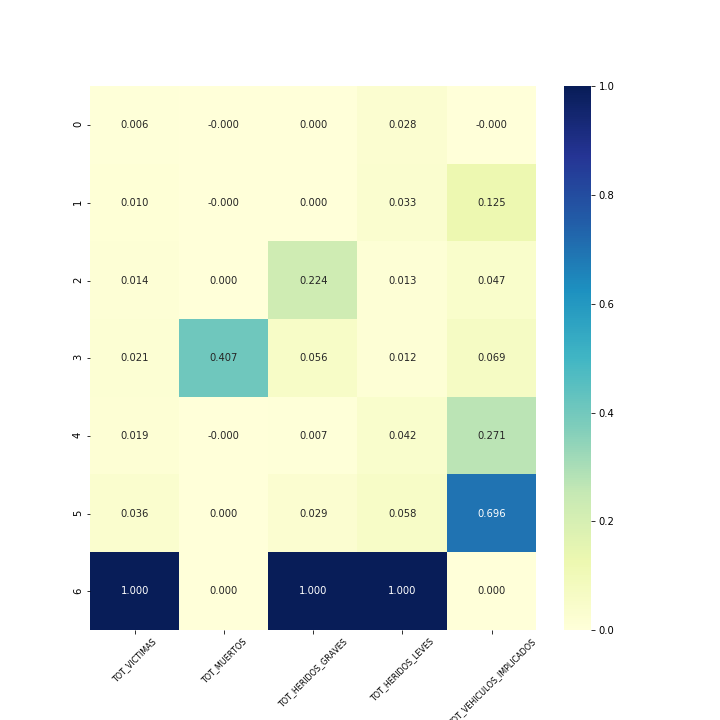
\includegraphics[width=0.9\textwidth]{imagenes/case1/kmeans/heatmaps/hm_kmeans_case1_salida_k7.png}
\end{subfigure}
\caption{Mapas de calor para el algoritmo K-Means, tipo 'enlace de salida'}
\label{fig:hm-km}
\end{figure}

\begin{figure}[H]
\begin{subfigure}{.5\textwidth}
  \centering
  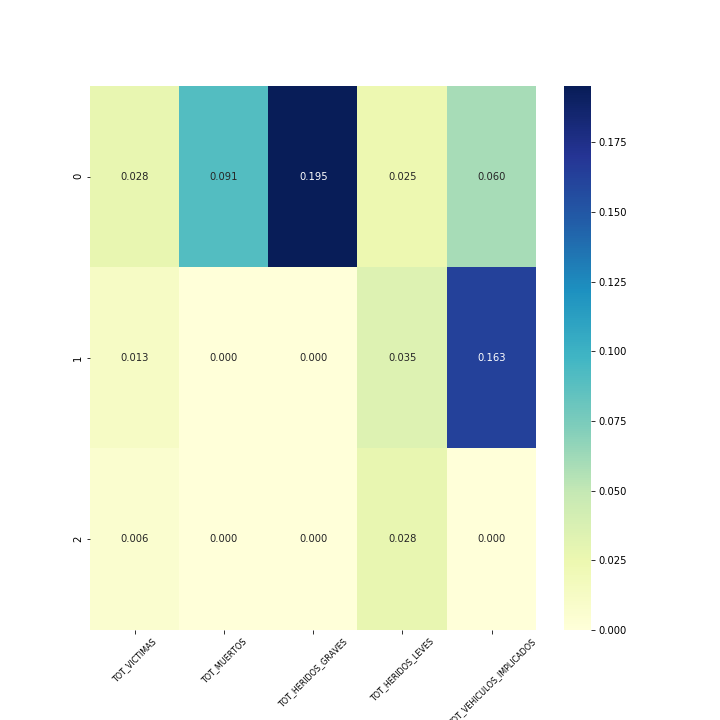
\includegraphics[width=0.9\textwidth]{imagenes/case1/agglomerative/heatmaps/hm_agglomerative_case1_salida_k3.png}
\end{subfigure}%
\begin{subfigure}{.5\textwidth}
  \centering
  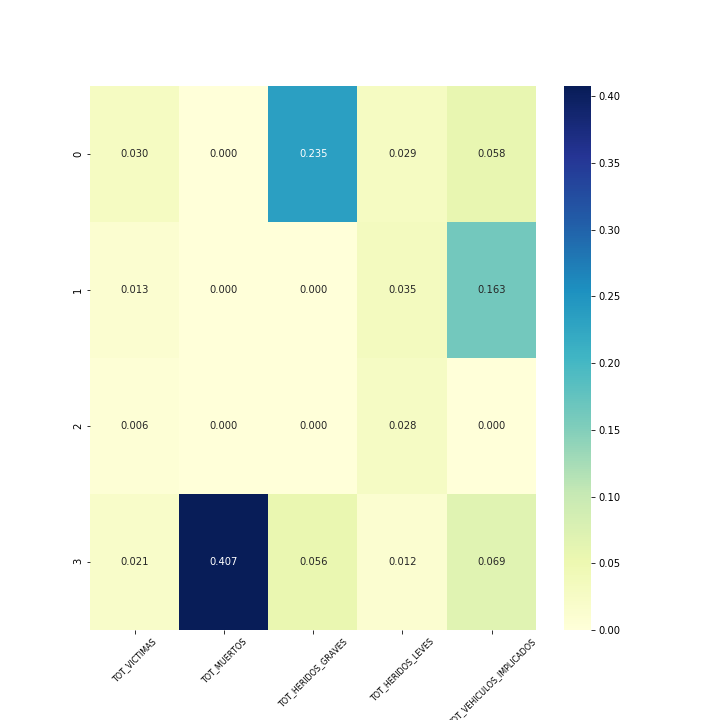
\includegraphics[width=0.9\textwidth]{imagenes/case1/agglomerative/heatmaps/hm_agglomerative_case1_salida_k4.png}
\end{subfigure}
\begin{subfigure}{.5\textwidth}
  \centering
  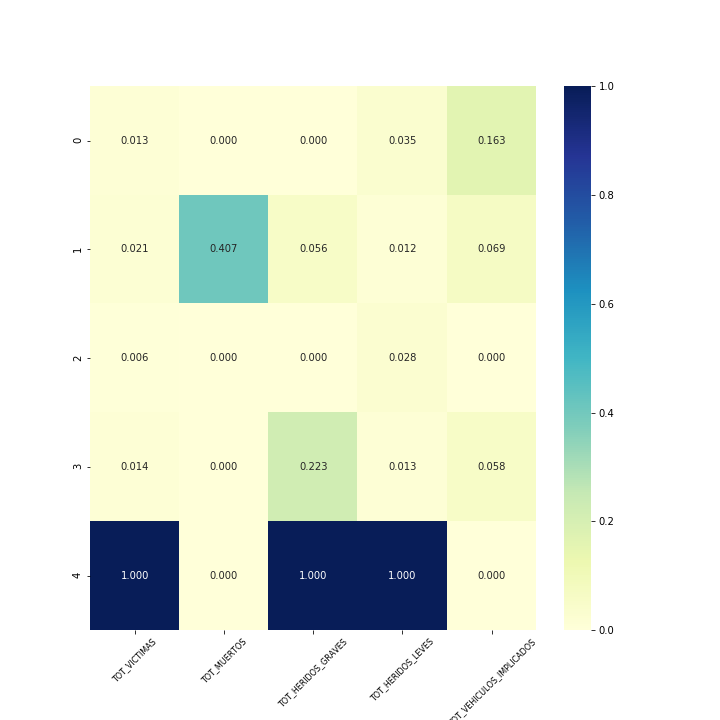
\includegraphics[width=0.9\textwidth]{imagenes/case1/agglomerative/heatmaps/hm_agglomerative_case1_salida_k5.png}
\end{subfigure}
\begin{subfigure}{.5\textwidth}
  \centering
  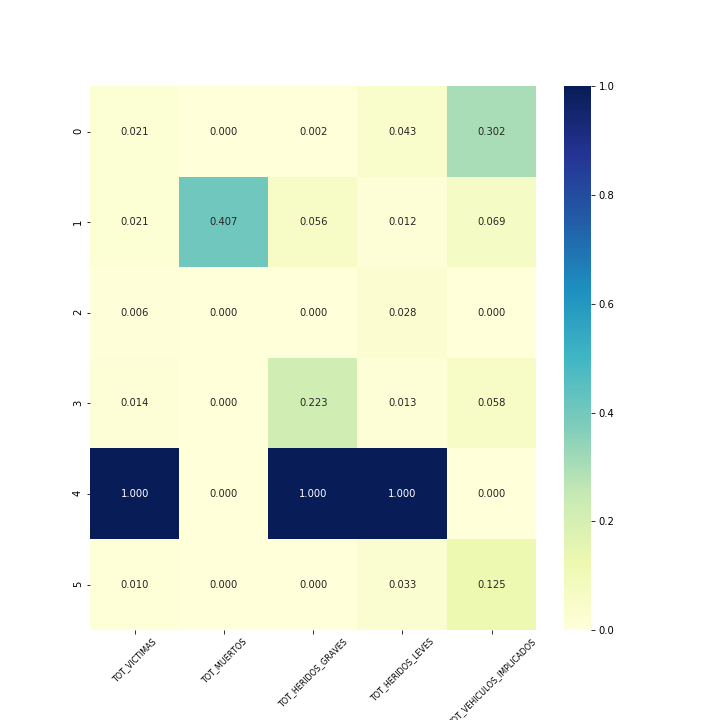
\includegraphics[width=0.9\textwidth]{imagenes/case1/agglomerative/heatmaps/hm_agglomerative_case1_salida_k6.png}
\end{subfigure}
\begin{subfigure}{.5\textwidth}
  \centering
  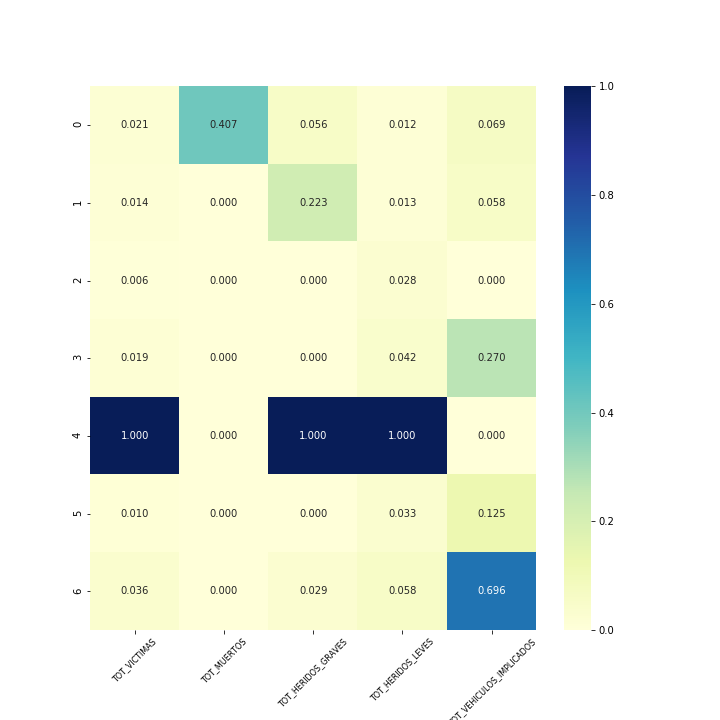
\includegraphics[width=0.9\textwidth]{imagenes/case1/agglomerative/heatmaps/hm_agglomerative_case1_salida_k7.png}
\end{subfigure}
\caption{Mapas de calor para el algoritmo Agglomerative Clustering, tipo 'enlace de salida'}
\label{fig:hm-km}
\end{figure}

\begin{figure}[H]
\begin{subfigure}{.5\textwidth}
  \centering
  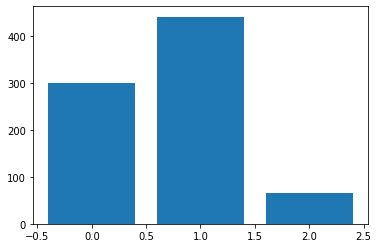
\includegraphics[width=0.45\textwidth]{imagenes/counter/salida/km3.png}
  \caption{$k=3$}
\end{subfigure}%
\begin{subfigure}{.5\textwidth}
  \centering
  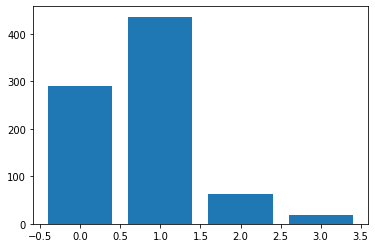
\includegraphics[width=0.45\textwidth]{imagenes/counter/salida/km4.png}
  \caption{$k=4$}
\end{subfigure}
\begin{subfigure}{.5\textwidth}
  \centering
  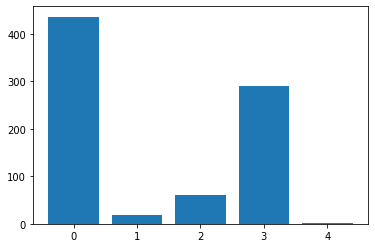
\includegraphics[width=0.45\textwidth]{imagenes/counter/salida/km5.png}
  \caption{$k=5$}
\end{subfigure}
\begin{subfigure}{.5\textwidth}
  \centering
  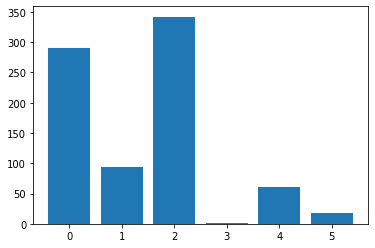
\includegraphics[width=0.45\textwidth]{imagenes/counter/salida/km6.png}
  \caption{$k=6$}
\end{subfigure}
\begin{subfigure}{.5\textwidth}
  \centering
  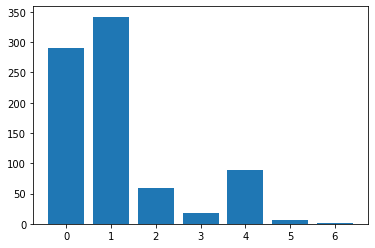
\includegraphics[width=0.45\textwidth]{imagenes/counter/salida/km7.png}
  \caption{$k=7$}
\end{subfigure}
\caption{Número de instancias en cada cluster(K-Means), tipo 'enlace de salida'}
\label{fig:hm-km}
\end{figure}


\begin{figure}[H]
\begin{subfigure}{.5\textwidth}
  \centering
  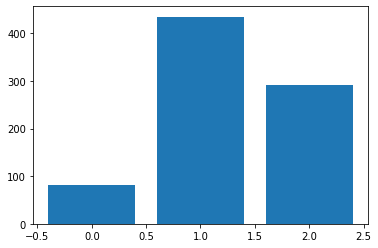
\includegraphics[width=0.45\textwidth]{imagenes/counter/salida/agg3.png}
  \caption{$k=3$}
\end{subfigure}%
\begin{subfigure}{.5\textwidth}
  \centering
  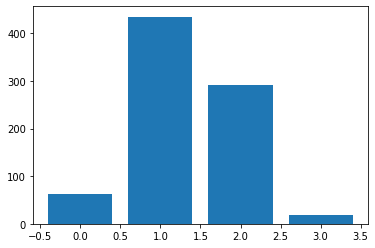
\includegraphics[width=0.45\textwidth]{imagenes/counter/salida/agg4.png}
  \caption{$k=4$}
\end{subfigure}
\begin{subfigure}{.5\textwidth}
  \centering
  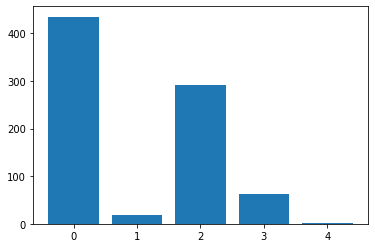
\includegraphics[width=0.45\textwidth]{imagenes/counter/salida/agg5.png}
  \caption{$k=5$}
\end{subfigure}
\begin{subfigure}{.5\textwidth}
  \centering
  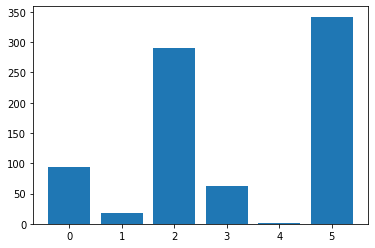
\includegraphics[width=0.45\textwidth]{imagenes/counter/salida/agg6.png}
  \caption{$k=6$}
\end{subfigure}
\begin{subfigure}{.5\textwidth}
  \centering
  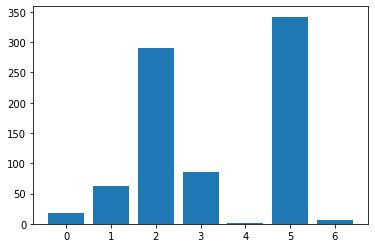
\includegraphics[width=0.45\textwidth]{imagenes/counter/salida/agg7.png}
  \caption{$k=7$}
\end{subfigure}
\caption{Número de instancias en cada cluster(Agglomerative-Clustering), tipo 'enlace de salida'}
\label{fig:hm-km}
\end{figure}

Por lo general en mi caso particular, hay muy pocas victimas por accidente y pocos heridos. Exceptuando un caso que parece ser de un accidente de un autobús por la cantidad de víctimas.

Se puede ver como uno de los clusters siempre tiene 1 vehículo implicado(posiblemente los atropellos y las colisiones con obstáculos) y otro con el valor máximo de victimas(52), con este último siempre estando solo en su cluster. También se ven los que tienen algunos vehículos implicados, que serán choques entre vehículos.

Las pocas cifras de muertos que hay, seguramente quedan en los clusters con muy pocas instancias en ellos, al igual que pasará con los heridos graves.

Como vista global, hay muchos menos heridos de los que me esperaba con mi primera hipótesis, así como obviamente mortalidad quedando agrupados los casos con un solo vehículo(atropellos) y el resto se forman dependiendo de los pocos heridos que haya o si algún vehículo ha estado implicado.

\subsubsection{Tipo de intersección - Enlace de entrada}

Ahora veremos el caso opuesto, las situaciones cuando se producen estos accidentes en las intersecciones de entrada.

En cuanto al tipo de vía sigue siendo la mayoría en autovía, pero en este caso también en autopista incluso superando a esta otra. También en las ramas de enlace se reduce mucho la cantidad de accidentes en comparación al caso opuesto, al igual que en vías de servicio.

\begin{figure}[H]
\centering
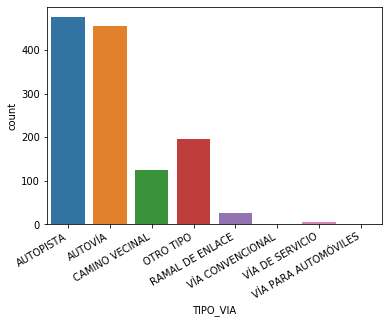
\includegraphics[width=0.5\textwidth]{imagenes/tipo_via_caso2.png}
\caption{Tipo de vía en intersecciones de tipo 'enlace de entrada'}
\end{figure}

El número de víctimas es casi igual al que hay en los enlaces de salida.

En cuanto al tipo de accidentes que se producen, se mantiene el dominio de los atropellos a animales seguido por peatones(aunque reducido con respecto al caso opuesto). Las colisiones con obstáculos se ve reducida(en bastante medida) y la colisión con vehículos se ve aumentada.

\begin{figure}[H]
\begin{subfigure}{.5\textwidth}
  \centering
  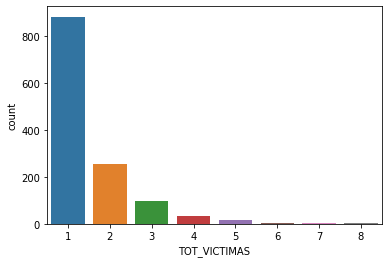
\includegraphics[width=0.8\textwidth]{imagenes/victimas_caso1-op.png}
  \caption{Número de victimas en intersecciones de tipo 'enlace de entrada'}
  \label{fig:sfig1}
\end{subfigure}%
\begin{subfigure}{.5\textwidth}
  \centering
  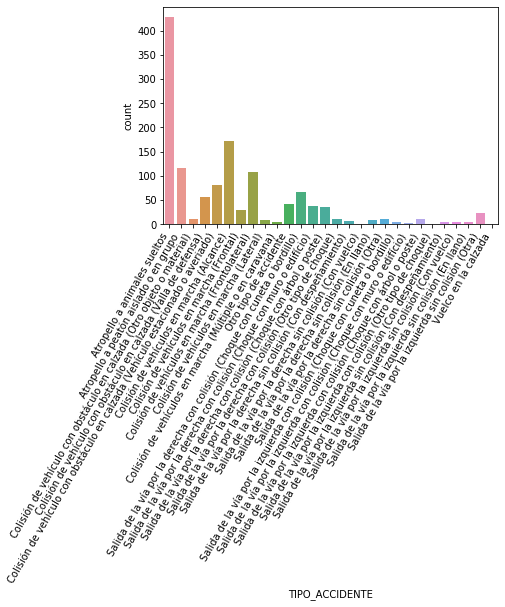
\includegraphics[width=0.8\textwidth]{imagenes/tipo_accidente_caso1-op.png}
  \caption{Tipo de accidentes en intersecciones de tipo 'enlace de entrada'}
  \label{fig:sfig2}
\end{subfigure}
\caption{Víctimas y tipos de accidente en intersecciones de tipo 'enlace de entrada'}
\label{fig:fig}
\end{figure}

\paragraph{Resultados de la segmentación}

Para evaluar la calidad del agrupamiento obtenido, se usarán las mismas medidas de evaluación que en el caso anterior.

\begin{table}[H]
%1
\begin{subtable}[H]{0.45\textwidth}
        \centering
\begin{tabular}{|c|c|c|}
\hline
\textit{k = 3}      & \textbf{K-Means}           & \textbf{Agg-Clustering} \\ \hline
\textbf{Silhouette} & \textit{\textbf{0,6001}}   & \textit{0,5951}         \\ \hline
\textbf{Calinski}   & \textit{\textbf{789,7076}} & 746,7932                \\ \hline
\end{tabular}
\end{subtable}
\hfill
\begin{subtable}[H]{0.45\textwidth}
        \centering
\begin{tabular}{|c|c|c|}
\hline
\textit{k = 4}      & \textbf{K-Means}           & \textbf{Agg-Clustering} \\ \hline
\textbf{Silhouette} & \textit{\textbf{0,5706}}   & \textit{0,5217}         \\ \hline
\textbf{Calinski}   & \textit{\textbf{818,6911}} & 689,6661                \\ \hline
\end{tabular}
\end{subtable}
%2
\begin{subtable}[H]{0.45\textwidth}
        \centering
\begin{tabular}{|c|c|c|}
\hline
\textit{k = 5}      & \textbf{K-Means}           & \textbf{Agg-Clustering} \\ \hline
\textbf{Silhouette} & \textit{\textbf{0,6568}}   & \textit{0,6238}         \\ \hline
\textbf{Calinski}   & \textit{\textbf{846,7492}} & 693,9017                \\ \hline
\end{tabular}
\end{subtable}
\hfill
\begin{subtable}[H]{0.45\textwidth}
        \centering
\begin{tabular}{|c|c|c|}
\hline
\textit{k = 6}      & \textbf{K-Means}           & \textbf{Agg-Clustering} \\ \hline
\textbf{Silhouette} & \textit{\textbf{0,6795}}   & \textit{0,6470}         \\ \hline
\textbf{Calinski}   & \textit{\textbf{824,9188}} & 739,5186                \\ \hline
\end{tabular}
\end{subtable}
%3
\begin{subtable}[H]{0.45\textwidth}
        \centering
\begin{tabular}{|c|c|c|}
\hline
\textit{k = 7}      & \textbf{K-Means}           & \textbf{Agg-Clustering} \\ \hline
\textbf{Silhouette} & \textit{\textbf{0,7088}}   & \textit{0,6663}         \\ \hline
\textbf{Calinski}   & \textit{\textbf{932,9841}} & 813,6500                \\ \hline
\end{tabular}
\end{subtable}
\hfill
\caption{Resultados obtenidos con los distintos algoritmos para las intersecciones de tipo 'enlace de entrada'}
\end{table}

Para este caso también dan valores parecidos para Silhouette y se mantiene el mismo patrón que en el caso opuesto, K-Means queda por encima(mejor agrupamiento global) que con Agglomerative-Clustering.

\paragraph{Interpretación de la segmentación}

\begin{figure}[H]
\begin{subfigure}{.5\textwidth}
  \centering
  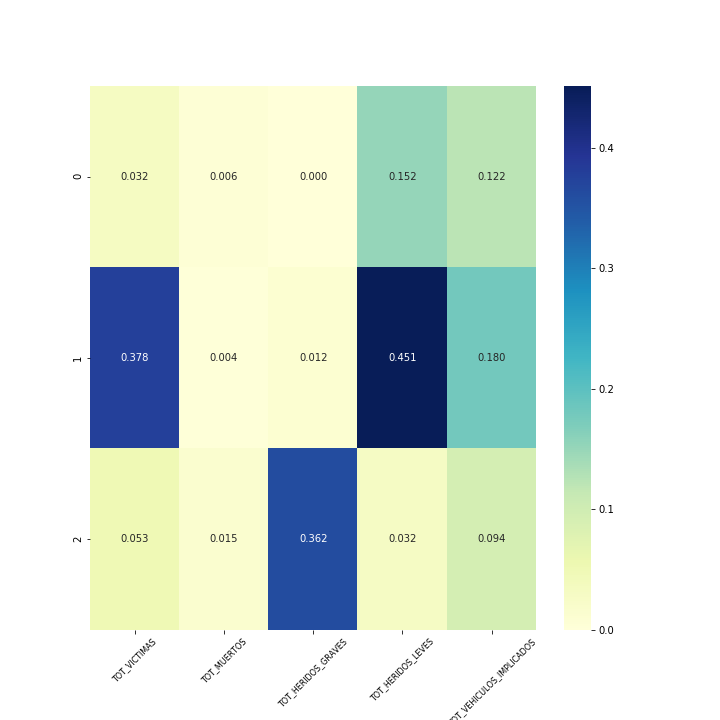
\includegraphics[width=0.9\textwidth]{imagenes/case1/kmeans/heatmaps/hm_kmeans_case1_entrada_k3.png}
\end{subfigure}%
\begin{subfigure}{.5\textwidth}
  \centering
  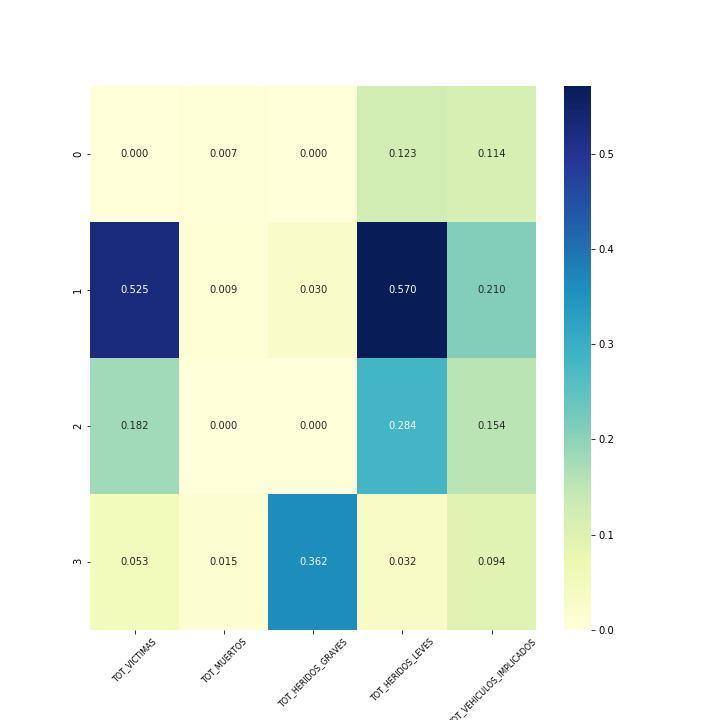
\includegraphics[width=0.9\textwidth]{imagenes/case1/kmeans/heatmaps/hm_kmeans_case1_entrada_k4.png}
\end{subfigure}
\begin{subfigure}{.5\textwidth}
  \centering
  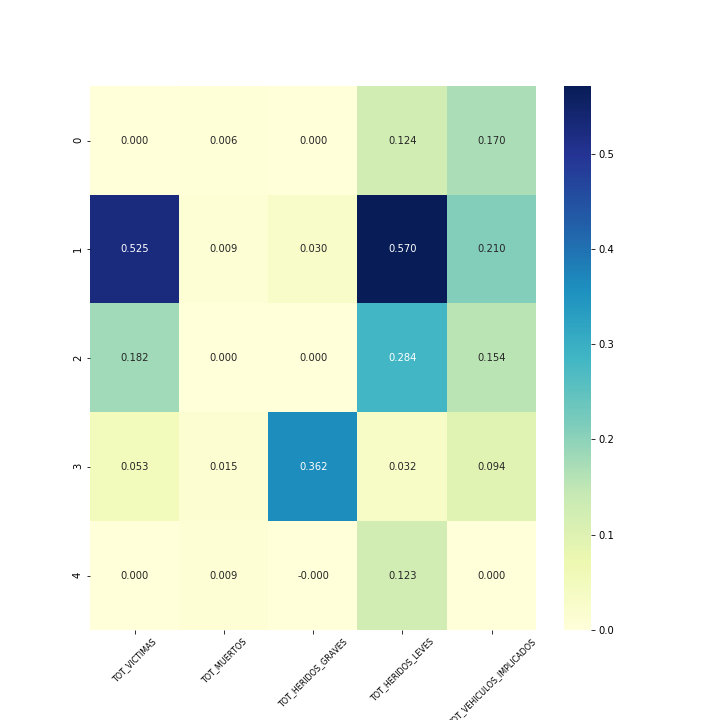
\includegraphics[width=0.9\textwidth]{imagenes/case1/kmeans/heatmaps/hm_kmeans_case1_entrada_k5.png}
\end{subfigure}
\begin{subfigure}{.5\textwidth}
  \centering
  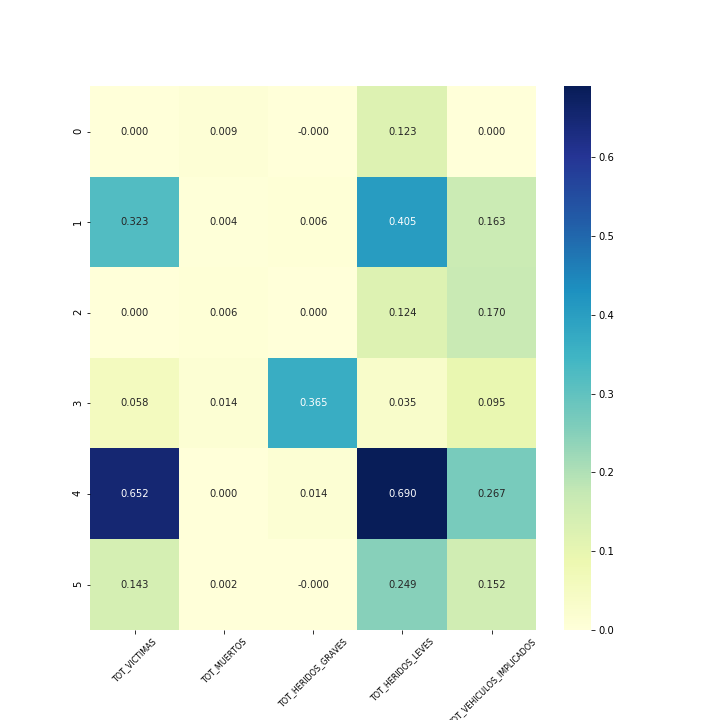
\includegraphics[width=0.9\textwidth]{imagenes/case1/kmeans/heatmaps/hm_kmeans_case1_entrada_k6.png}
\end{subfigure}
\begin{subfigure}{.5\textwidth}
  \centering
  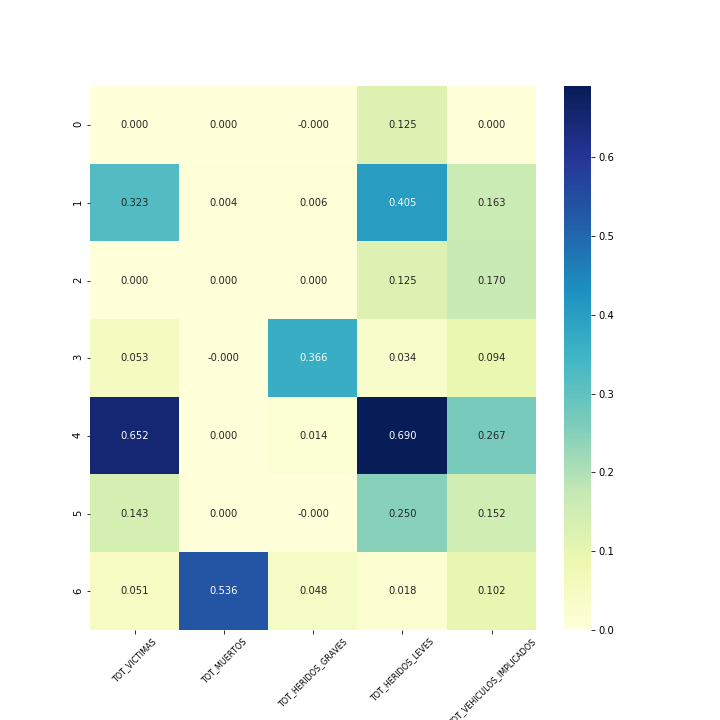
\includegraphics[width=0.9\textwidth]{imagenes/case1/kmeans/heatmaps/hm_kmeans_case1_entrada_k7.png}
\end{subfigure}
\caption{Mapas de calor para el algoritmo K-Means, tipo 'enlace de entrada'}
\label{fig:hm-km}
\end{figure}

\begin{figure}[H]
\begin{subfigure}{.5\textwidth}
  \centering
  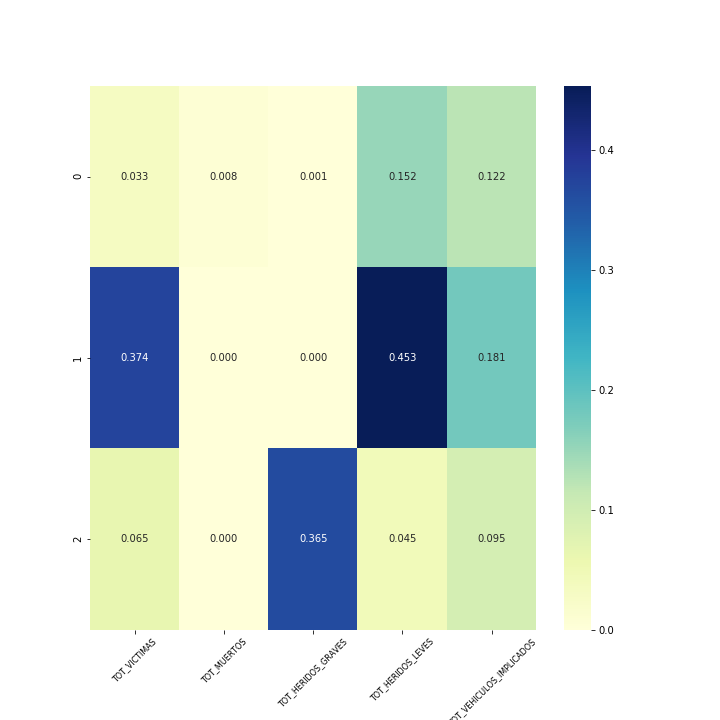
\includegraphics[width=0.9\textwidth]{imagenes/case1/agglomerative/heatmaps/hm_agglomerative_case1_entrada_k3.png}
\end{subfigure}%
\begin{subfigure}{.5\textwidth}
  \centering
  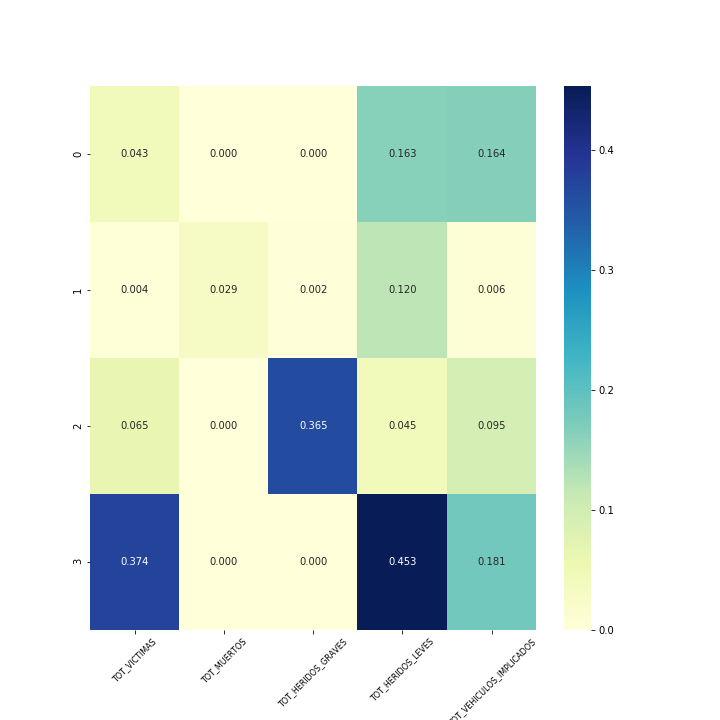
\includegraphics[width=0.9\textwidth]{imagenes/case1/agglomerative/heatmaps/hm_agglomerative_case1_entrada_k4.png}
\end{subfigure}
\begin{subfigure}{.5\textwidth}
  \centering
  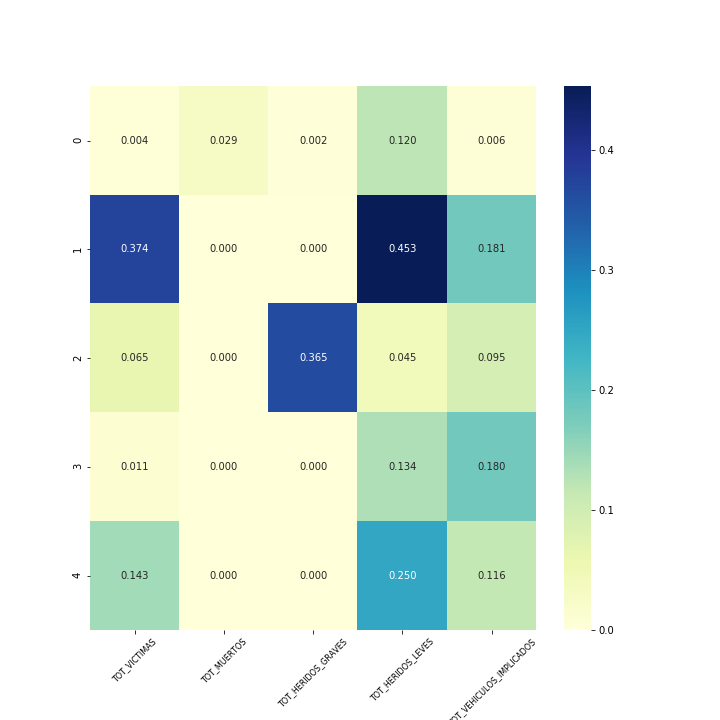
\includegraphics[width=0.9\textwidth]{imagenes/case1/agglomerative/heatmaps/hm_agglomerative_case1_entrada_k5.png}
\end{subfigure}
\begin{subfigure}{.5\textwidth}
  \centering
  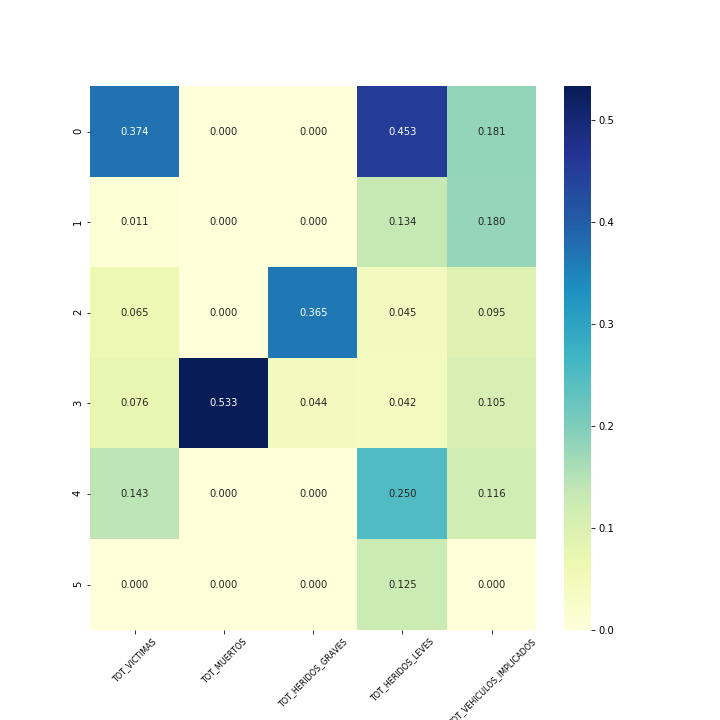
\includegraphics[width=0.9\textwidth]{imagenes/case1/agglomerative/heatmaps/hm_agglomerative_case1_entrada_k6.png}
\end{subfigure}
\begin{subfigure}{.5\textwidth}
  \centering
  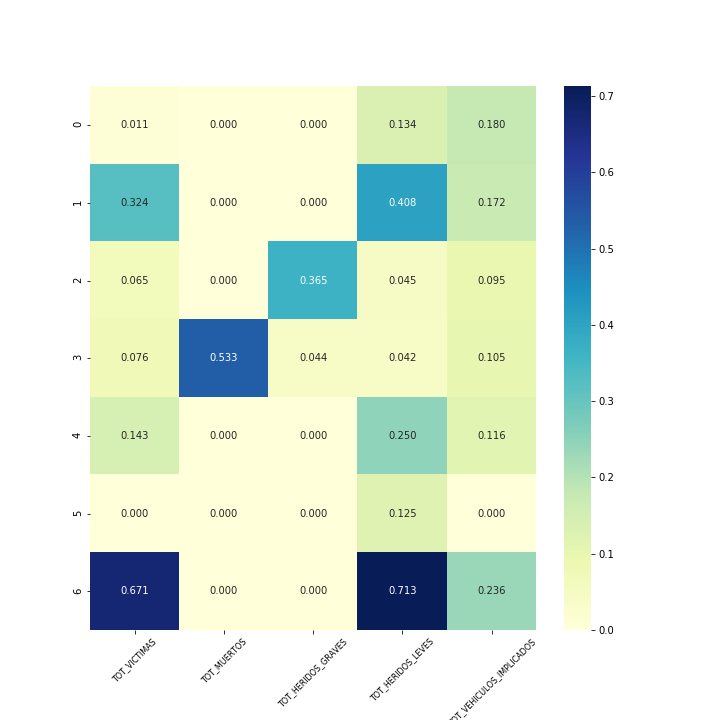
\includegraphics[width=0.9\textwidth]{imagenes/case1/agglomerative/heatmaps/hm_agglomerative_case1_entrada_k7.png}
\end{subfigure}
\caption{Mapas de calor para el algoritmo Agglomerative Clustering, tipo 'enlace de entrada'}
\label{fig:hm-km}
\end{figure}

\begin{figure}[H]
\begin{subfigure}{.5\textwidth}
  \centering
  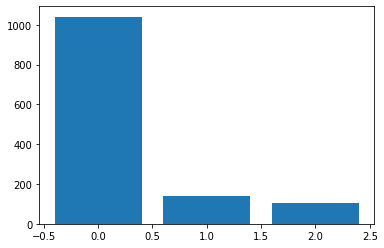
\includegraphics[width=0.45\textwidth]{imagenes/counter/entrada/km3.png}
  \caption{$k=3$}
\end{subfigure}%
\begin{subfigure}{.5\textwidth}
  \centering
  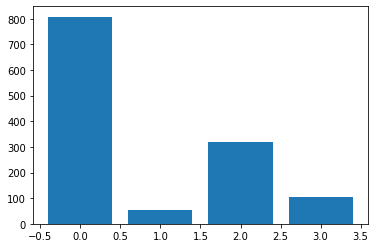
\includegraphics[width=0.45\textwidth]{imagenes/counter/entrada/km4.png}
  \caption{$k=4$}
\end{subfigure}
\begin{subfigure}{.5\textwidth}
  \centering
  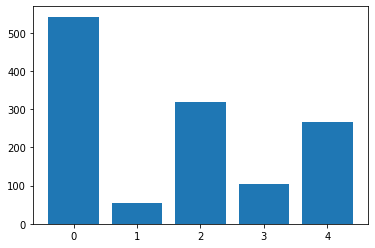
\includegraphics[width=0.45\textwidth]{imagenes/counter/entrada/km5.png}
  \caption{$k=5$}
\end{subfigure}
\begin{subfigure}{.5\textwidth}
  \centering
  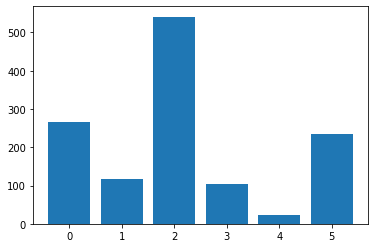
\includegraphics[width=0.45\textwidth]{imagenes/counter/entrada/km6.png}
  \caption{$k=6$}
\end{subfigure}
\begin{subfigure}{.5\textwidth}
  \centering
  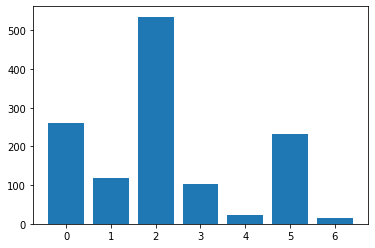
\includegraphics[width=0.45\textwidth]{imagenes/counter/entrada/km7.png}
  \caption{$k=7$}
\end{subfigure}
\caption{Número de instancias en cada cluster(K-Means), tipo 'enlace de entrada'}
\label{fig:hm-km}
\end{figure}

\begin{figure}[H]
\begin{subfigure}{.5\textwidth}
  \centering
  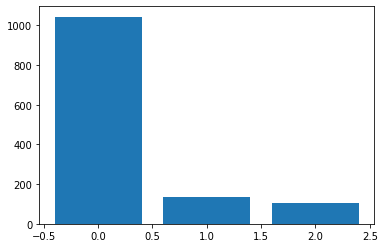
\includegraphics[width=0.45\textwidth]{imagenes/counter/entrada/agg3.png}
  \caption{$k=3$}
\end{subfigure}%
\begin{subfigure}{.5\textwidth}
  \centering
  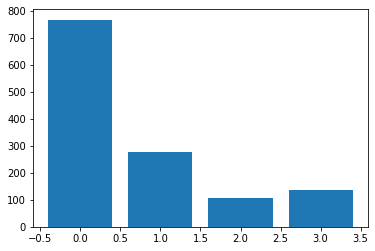
\includegraphics[width=0.45\textwidth]{imagenes/counter/entrada/agg4.png}
  \caption{$k=4$}
\end{subfigure}
\begin{subfigure}{.5\textwidth}
  \centering
  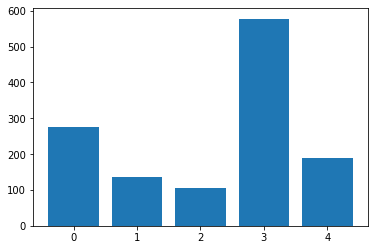
\includegraphics[width=0.45\textwidth]{imagenes/counter/entrada/agg5.png}
  \caption{$k=5$}
\end{subfigure}
\begin{subfigure}{.5\textwidth}
  \centering
  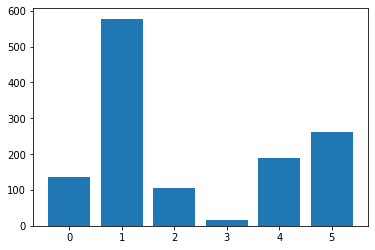
\includegraphics[width=0.45\textwidth]{imagenes/counter/entrada/agg6.png}
  \caption{$k=6$}
\end{subfigure}
\begin{subfigure}{.5\textwidth}
  \centering
  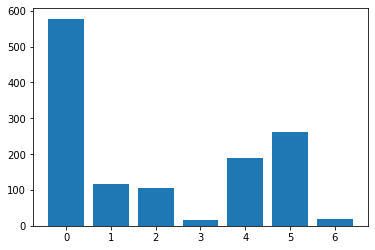
\includegraphics[width=0.45\textwidth]{imagenes/counter/entrada/agg7.png}
  \caption{$k=7$}
\end{subfigure}
\caption{Número de instancias en cada cluster(Agglomerative-Clustering), tipo 'enlace de entrada'}
\label{fig:hm-km}
\end{figure}

En este caso parece apreciarse como ya aparecen más víctimas y heridos que en el caso anterior(seguramente sea por el aumento de colisiones con vehículos).

Vuelve a aparecer un cluster cuando aumenta el valor de $k$ con un solo vehículo implicado de media(atropellos), y termina agrupandose a los pocos accidentes con casos mortales en un cluster en su mayoría. 

Los clusters parecen mantenerse conforme aumenta la $k$ formándose otros nuevos para especificar más.

Como conclusión, aparece un aumento de heridos(tanto leves como graves) y de víctimas totales.
